\documentclass[10pt]{beamer}
\usetheme{Madrid}
\usepackage{booktabs}
\usepackage{graphicx}
\usepackage[T1]{fontenc}
\usepackage{tikz}
\usetikzlibrary{arrows.meta}
\setbeamertemplate{navigation symbols}{}
% To view speaker notes, uncomment the next line (adds note pages):
% \setbeameroption{show notes}
\tikzset{
  box/.style={draw, rounded corners, align=center, text width=2.3cm, minimum height=0.9cm, font=\scriptsize},
  kuser/.style={box, fill=blue!15}, kagent/.style={box, fill=green!25},
  kdata/.style={box, fill=black!8}, kdanger/.style={box, fill=red!25},
  koutput/.style={box, fill=orange!25}, kdecision/.style={box, fill=yellow!30},
  kguard/.style={box, fill=violet!25},
  flow/.style={-{Stealth[length=2mm]}, thick},
}
% ======================= EDIT YOUR DETAILS =======================
\newcommand{\studentname}{Aflah Muhammed P}
% Change the university roll/registration number:
\newcommand{\rollno}{TVE23CSXXX}
% Change your class roll number:
\newcommand{\rollclass}{Roll No: XX}
% Change your guide name:
\newcommand{\guidename}{Prof. Guide Name}
% Change department / college / short-institute if needed:
\newcommand{\deptname}{Department of Computer Science and Engineering}
\newcommand{\collegename}{College of Engineering Trivandrum}
\newcommand{\shortinst}{CET}
% Change the seminar date:
\newcommand{\seminardate}{\today}
% =================================================================
\title[B.Tech Seminar]{Can We Trust AI Agents? A Beginner's Map of Threats and Defenses (TrustAgent)}
\subtitle{Based on: A Survey on Trustworthy LLM Agents: Threats and Countermeasures (arXiv:2503.09648, 2025)}
\author[\studentname\ (\shortinst)]{\studentname \\ \small \rollno \\ \small \rollclass \\ \small Guide: \guidename}
\institute[]{\deptname \\ \collegename}
\date{\seminardate}
\begin{document}
\begin{frame}[plain]
  \titlepage
\end{frame}
\begin{frame}{Table of Contents}
  \tableofcontents
\end{frame}
\section{Introduction}
\begin{frame}{Introduction}
\begin{itemize}
  \item LLM agents extend chatbots with memory, tools, and real actions.
  \item Multi-agent systems let several agents cooperate, compete, or debate.
  \item More capability also means a much larger attack surface.
  \item Trustworthiness spans safety, privacy, truthfulness, fairness, and robustness.
  \item This survey introduces TrustAgent, a unified map of agent threats.
  \item It organizes attacks, defenses, and evaluation across six agent modules.
\end{itemize}
\end{frame}
\note{Start friendly: an AI agent is a chatbot that can also remember things, use tools, and take actions in the world. When several of them work together we call it a multi-agent system. All that extra power creates new ways to be attacked, so we need to ask whether we can trust these agents. This talk walks through one clear map of the threats and the defenses.}
\section{Literature Survey}
\begin{frame}{Literature Survey / Background}
  \small
  \begin{tabular}{@{}p{2.7cm}p{2.3cm}p{5.6cm}@{}}
    \toprule
    \textbf{Title} & \textbf{Author} & \textbf{Summary} \\
    \midrule
    TrustLLM: Trustworthiness in Large Language Models & Huang et al. (2024) & Benchmarks LLM trustworthiness across six perspectives, but targets standalone models, not agents with memory, tools, or peer agents. \\
    \addlinespace
    The Emerged Security and Privacy of LLM Agent: A Survey with Case Studies & He et al. (2024) & Reviews agent security and privacy through case studies, focusing mainly on the LLM brain rather than all modules. \\
    \addlinespace
    Navigating the Risks: Security, Privacy, and Ethics Threats in LLM-Based Agents & Gan et al. (2024) & Surveys agent security, privacy, and ethics threats, but largely omits defenses and evaluation and overlaps with LLM work. \\
    \addlinespace
    \bottomrule
  \end{tabular}
\end{frame}
\note{Earlier work mostly studied trustworthiness of plain language models, like the TrustLLM benchmark. A couple of agent surveys came later, but they focused narrowly on the brain, or on threats without defenses. Point out that this paper is the first to cover the whole picture: brain, memory, tools, and interactions, with attacks, defenses, and evaluation together.}
\section{Motivation}
\begin{frame}{Motivation}
\begin{itemize}
  \item Agents bolt memory, tools, environments, and other agents onto LLMs.
  \item Each added module opens a fresh door for attackers.
  \item Safety research on LLMs alone misses these agent-specific risks.
  \item Attacks can now spread between agents like a contagion.
  \item Real actions like driving or payments make failures genuinely costly.
\end{itemize}
\end{frame}
\note{Explain the double-edged sword idea: bolting on memory, tools, and other agents makes systems smarter but adds more doors for attackers. Old safety research assumed a single, isolated model, so it misses these new risks. Stress that agents now take real actions, like driving or making payments, so mistakes can cause real harm.}
\section{Problem Statement}
\begin{frame}{Problem Statement}
  \begin{block}{}
  As LLMs gain memory, tools, environments, and peer agents, entirely new trustworthiness risks appear that LLM-only safety research does not cover. No prior survey jointly maps these agent and multi-agent threats together with their matching defenses and evaluation methods.
  \end{block}
\end{frame}
\note{Say plainly that the field had no single framework tying agent threats to their defenses and tests. Each new module, memory, tools, environment, other agents, brings risks nobody had organized. This survey sets out to fill that gap with one shared vocabulary.}
\section{Objectives}
\begin{frame}{Objectives}
\begin{itemize}
  \item Extend trustworthy-LLM ideas to agents and multi-agent systems.
  \item Deconstruct an agent into six internal and external modules.
  \item Categorize threats by safety, privacy, truthfulness, fairness, and robustness.
  \item Summarize attacks, defenses, and evaluation methods per module.
  \item Identify current research gaps and promising future directions.
  \item Provide a public, categorized reference repository for the community.
\end{itemize}
\end{frame}
\note{Tell the audience what the authors set out to do: extend LLM trust ideas to agents, break an agent into six parts, and study each part for attacks, defenses, and evaluation. They also flag where research is missing and share a public list of papers. Keep it as a simple checklist of goals.}
\section{Methodology}
\begin{frame}[allowframebreaks]{Methodology: Intrinsic Trustworthiness: Brain, Memory, Tools}
\begin{itemize}
  \item Brain is the LLM core; hit by jailbreak, prompt injection, backdoor.
  \item Memory covers RAG vector stores and dialogue history; risks poisoning and leakage.
  \item Tools are APIs, sensors, and robots; risks manipulation and abuse.
  \item Defenses include alignment, input and output filters, and guard agents.
\end{itemize}
\end{frame}
\note{Walk through the framework in three easy pieces. First, intrinsic parts inside the agent: the brain, its memory, and its tools. Second, extrinsic interactions with other agents, the environment, and the user. Third, for every part they ask the same three questions: how is it attacked, how is it defended, and how do we measure it.}
\begin{frame}[allowframebreaks]{Methodology: Extrinsic Trustworthiness: Agents, Environment, Users}
\begin{itemize}
  \item Agent-to-agent: cooperative and infectious attacks spread across the system.
  \item Agent-to-environment: physical risks (robots, cars) and digital risks (web, finance).
  \item Agent-to-user: trust calibration, transparency, and personalization concerns.
  \item Defenses use debate, voting, and graph-based topology checks.
\end{itemize}
\end{frame}
\begin{frame}[allowframebreaks]{Methodology: Three Technical Lenses: Attack, Defense, Evaluation}
\begin{itemize}
  \item Attack: how each module can be compromised.
  \item Defense: countermeasures that protect each module.
  \item Evaluation: benchmarks and metrics that measure trustworthiness.
  \item Applied uniformly across all six modules for fair comparison.
\end{itemize}
\end{frame}
\section{Key Concepts}
\begin{frame}[allowframebreaks]{Key Concepts}
  \begin{description}
    \item[LLM Agent] An LLM brain extended with memory, tools, and the ability to act on an environment.
    \item[Multi-agent System (MAS)] Several agents communicating to cooperate, compete, or debate toward a shared task.
    \item[Intrinsic vs Extrinsic] Internal parts (brain, memory, tools) versus external interactions (users, other agents, environment).
    \item[Jailbreak] Crafted prompts that bypass an agent's safety alignment to force harmful output.
    \item[Prompt Injection] Hidden malicious instructions inside data that override the agent's original task.
    \item[Memory Poisoning] Injecting malicious documents into a database so retrieval misleads the agent.
  \end{description}
\end{frame}
\note{Define the jargon before diving deeper. An agent is an LLM plus memory, tools, and actions; a multi-agent system is several agents talking to each other. Then explain three attacks in plain words: jailbreak tricks the safety rules, prompt injection hides sneaky instructions in data, and memory poisoning plants bad documents the agent later trusts.}
\section{System Architecture}
\begin{frame}{System Architecture}
  \begin{center}
  \resizebox{0.96\textwidth}{!}{%
  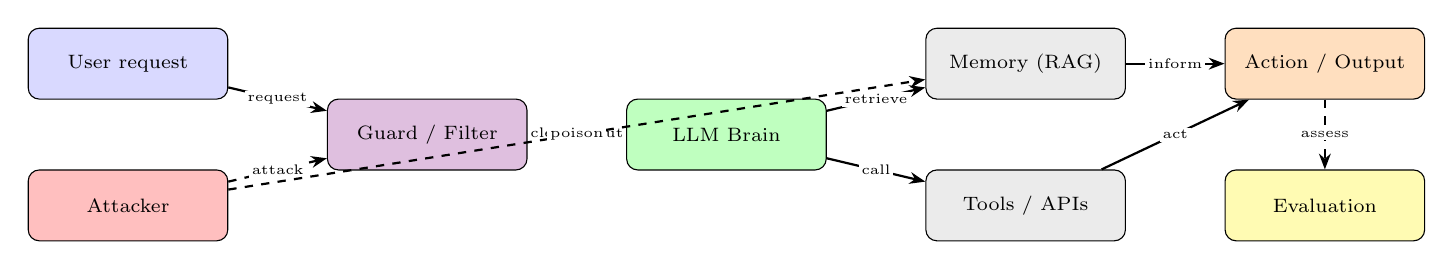
\begin{tikzpicture}
    \node[kuser] (user) at (0.00,0.90) {User request};
    \node[kdanger] (attacker) at (0.00,-0.90) {Attacker};
    \node[kguard] (guard) at (3.80,0.00) {Guard / Filter};
    \node[kagent] (brain) at (7.60,0.00) {LLM Brain};
    \node[kdata] (memory) at (11.40,0.90) {Memory (RAG)};
    \node[kdata] (tools) at (11.40,-0.90) {Tools / APIs};
    \node[koutput] (output) at (15.20,0.90) {Action / Output};
    \node[kdecision] (eval) at (15.20,-0.90) {Evaluation};
    \draw[flow] (user) -- (guard) node[midway, font=\tiny, fill=white, inner sep=1pt]{request};
    \draw[flow, dashed] (attacker) -- (guard) node[midway, font=\tiny, fill=white, inner sep=1pt]{attack};
    \draw[flow] (guard) -- (brain) node[midway, font=\tiny, fill=white, inner sep=1pt]{clean input};
    \draw[flow] (brain) -- (memory) node[midway, font=\tiny, fill=white, inner sep=1pt]{retrieve};
    \draw[flow] (brain) -- (tools) node[midway, font=\tiny, fill=white, inner sep=1pt]{call};
    \draw[flow, dashed] (attacker) -- (memory) node[midway, font=\tiny, fill=white, inner sep=1pt]{poison};
    \draw[flow] (memory) -- (output) node[midway, font=\tiny, fill=white, inner sep=1pt]{inform};
    \draw[flow] (tools) -- (output) node[midway, font=\tiny, fill=white, inner sep=1pt]{act};
    \draw[flow, dashed] (output) -- (eval) node[midway, font=\tiny, fill=white, inner sep=1pt]{assess};
  \end{tikzpicture}%
  }
  \end{center}
  \begin{center}\scriptsize A user request flows through a guard into the agent's brain, memory, and tools, while attackers target each stage and evaluation checks the output.\end{center}
\end{frame}
\note{Use the diagram as a story from left to right. A user request and an attacker's malicious input both arrive, and a guard tries to filter them. The clean request reaches the brain, which pulls facts from memory and calls tools to act. Point at the dashed red arrows: those are attacks sneaking in, and evaluation at the end double-checks the output.}
\begin{frame}[allowframebreaks]{How It Works (Explained)}
\begin{itemize}
  \item On the left a user sends a normal request while an attacker sends malicious input.
  \item A guard or filter screens incoming prompts before they reach the agent.
  \item The cleaned request enters the LLM brain, the reasoning and decision center.
  \item The brain retrieves facts from memory and calls tools or APIs to act.
  \item Dashed arrows show attacks: injection at the input and poisoning into memory.
  \item The resulting action or output is checked by evaluation before returning to the user.
\end{itemize}
\end{frame}
\section{Example Walkthrough}
\begin{frame}[allowframebreaks]{Example Walkthrough: Tracing a memory-poisoning attack and its defense}
\begin{enumerate}
  \item A user asks a shopping assistant for the safest product to buy.
  \item The agent's brain queries its long-term memory, a vector database.
  \item Earlier, an attacker injected a malicious document (PoisonedRAG) into that database.
  \item The poisoned text ranks high and is retrieved as context.
  \item Without defense, the brain repeats the false, unsafe recommendation.
  \item A detection defense (TrustRAG) clusters retrieved documents and drops the outlier.
  \item The cleaned context now yields a safe, truthful answer to the user.
\end{enumerate}
\end{frame}
\note{Ground everything in one concrete example a beginner can picture. A shopping assistant looks up product info in its memory database, but an attacker planted a fake document there earlier. Without protection the agent gives a false, unsafe answer. Then show the fix: a detection defense spots the odd document, removes it, and the user gets a safe answer.}
\section{Results}
\begin{frame}[allowframebreaks]{Results / Findings}
\begin{itemize}
  \item First survey to jointly cover LLM, agent, and MAS with attack, defense, and evaluation together (Table 1).
  \item Organizes threats across 6 modules and 5 trustworthiness dimensions.
  \item Brain module alone catalogs 3 attack types, 3 defense types, and 2 evaluation types.
  \item AgentHarm benchmark spans 110 malicious agent tasks across fraud, cybercrime, and harassment.
  \item R-Judge uses 27 risk scenarios; S-Eval spans 8 risk dimensions across 4 levels.
  \item Agent Smith shows one adversarial image can jailbreak about one million agents exponentially fast.
\end{itemize}
\end{frame}
\note{Highlight that this is the first survey to combine models, single agents, and multi-agent systems with attacks, defenses, and evaluation in one map. Share a few concrete numbers so it feels real: the AgentHarm benchmark has 110 malicious tasks, R-Judge covers 27 risk scenarios, and one clever image attack spread to around a million agents. These show the threats are already large and measurable.}
\section{Discussion}
\begin{frame}{Discussion}
\begin{itemize}
  \item Adding modules boosts capability (MAS beats single agent beats plain LLM) but enlarges the attack surface.
  \item Attacks now propagate between agents (infectious attacks), a threat absent in single LLMs.
  \item Defenses and evaluation clearly lag behind attacks, especially for tools and memory.
  \item Agent-to-user trust, transparency, and calibration remain largely underexplored.
\end{itemize}
\end{frame}
\note{Make the trade-off clear: more modules mean smarter agents but bigger attack surfaces. The scariest new twist is that attacks can now jump from one agent to another, something a lone chatbot never faced. Note that defenses and tests are still catching up, especially for tools and memory.}
\section{Challenges}
\begin{frame}{Limitations \& Challenges}
\begin{itemize}
  \item A snapshot of a fast-moving field; new attacks appear after March 2025.
  \item The survey synthesizes and categorizes prior work rather than running new experiments.
  \item Some modules (tool defense, memory evaluation) have too few papers to generalize.
  \item The agent-to-user section is mostly discussion, lacking concrete techniques.
\end{itemize}
\end{frame}
\note{Be honest that this is a survey, not new experiments, and the field moves fast, so newer attacks already exist. Some areas, like defending tools, have very few papers, so conclusions there are tentative. The user-interaction section is mostly discussion rather than concrete methods.}
\section{Future Work}
\begin{frame}{Future Work}
\begin{itemize}
  \item Build collaborative, consensus-based defenses so agents verify each other's actions.
  \item Move from static datasets to dynamic, real-time evaluation environments.
  \item Develop tool-invocation defenses and database-side poisoning prevention.
  \item Create adaptive trust-calibration and explainable agents for end users.
\end{itemize}
\end{frame}
\note{Point to the exciting open problems: let agents watch and verify each other, test them in live changing environments instead of fixed datasets, and finally build real defenses for tools and databases. Also mention making agents explain themselves so users can calibrate how much to trust them.}
\section{Conclusion}
\begin{frame}{Conclusion}
\begin{itemize}
  \item TrustAgent unifies agent trustworthiness into a modular, technical, multi-dimensional taxonomy.
  \item It maps attacks, defenses, and evaluations across six internal and external modules.
  \item It highlights urgent gaps: tool defense and memory and inter-agent evaluation.
  \item The goal is to guide safer development of agents and multi-agent systems.
\end{itemize}
\end{frame}
\note{Wrap up by restating the big idea: TrustAgent gives one clean map of agent trustworthiness across six modules and three lenses. It shows where we are protected and, importantly, where we are not, like tool defense and memory testing. Leave the audience with the takeaway that building trustworthy agents is an urgent, shared task.}
\section{References}
\begin{frame}[allowframebreaks]{References}
  \footnotesize
  \begin{enumerate}
    \item Yu, M., Meng, F., Zhou, X., Wang, S., Mao, J., Pang, L., Chen, T., Wang, K., Li, X., Zhang, Y., An, B., Wen, Q. (2025). A Survey on Trustworthy LLM Agents: Threats and Countermeasures. arXiv:2503.09648 (KDD 2025).
    \item Huang, Y., Sun, L., Wang, H., Wu, S., Zhang, Q., et al. (2024). TrustLLM: Trustworthiness in Large Language Models. arXiv:2401.05561.
    \item He, F., Zhu, T., Ye, D., Liu, B., Zhou, W., Yu, P. S. (2024). The Emerged Security and Privacy of LLM Agent: A Survey with Case Studies. arXiv:2407.19354.
    \item Gan, Y., Yang, Y., Ma, Z., He, P., Zeng, R., et al. (2024). Navigating the Risks: A Survey of Security, Privacy, and Ethics Threats in LLM-Based Agents. arXiv:2411.09523.
    \item Andriushchenko, M., Souly, A., Dziemian, M., et al. (2024). AgentHarm: A Benchmark for Measuring Harmfulness of LLM Agents. arXiv:2410.09024.
    \item Chen, Z., Xiang, Z., Xiao, C., Song, D., Li, B. (2025). AgentPoison: Red-teaming LLM Agents via Poisoning Memory or Knowledge Bases. NeurIPS 2024.
  \end{enumerate}
\end{frame}
\begin{frame}[plain]
  \begin{center}
    {\Huge Thank You}\\[1em]
    {\large Questions?}
  \end{center}
\end{frame}
\end{document}